%% ------------------------------------------------------------------------- %%
\chapter{Introdução}
\label{cap:introducao}

O software é ubíquo na sociedade moderna. Está presente praticamente em todas as atividades do cotidiano, seja no transporte, na medicina, finanças e até mesmo entretenimento, que dependem de um software de alta qualidade que esteja funcionando corretamente e seja confiável. O desenvolvimento de software é uma tarefa onerosa: desenvolvedores devem lidar com a complexidade de um software, enquanto tentam evitar erros, e ainda assim devem entregar o produto a tempo e com qualidade. Além disso, há uma demanda contínua por inovação nas ferramentas de software que ajudam a desenvolver software mais confiável e fácil de manter. Novos métodos são constantemente procurados para reduzir a complexidade do software e ajudar os desenvolvedores a construir um software melhor \citep{Allamanis:2018:SML}.

Além de novos métodos e ferramentas, um outro aliado dos desenvolvedores são os fóruns de dúvidas de programação. Nestes fóruns, desenvolvedores fazem perguntas a respeito de problemas específicos de programação, algoritmos, ferramentas para desenvolvimento e práticas comuns de desenvolvimento software \citep{stackoverflow-questions-topics-2019}. Um importante fórum de dúvidas de programação é o \Gls{sof}. De acordo com o último relatório, 50 milhões de pessoas visitam o site \Gls{sof} por mês. E destes 50 milhões, 21 milhões são estudantes universitários ou desenvolvedores profissionais \citep{stackoverflow-survey-2019}.

O \Gls{sof} contém mais de 1 milhão e 200 mil perguntas relacionadas a linguagem Python (Figura~\ref{fig:bigquery-total-questions-python-stackoverflow}). No total, há mais de 17 milhões de dúvidas publicadas no site até o dia 11 de junho de 2019 (Figura~\ref{fig:bigquery-total-questions-stackoverflow}). O benefício de plataformas abertas de perguntas e respostas como o \textit{Stackoverflow} ou \textit{Quora}\footnote{Quora é um website de perguntas e respostas onde as perguntas são feitas, respondidas, editadas e organizadas por sua comunidade de usuários \citep{wikipedia-quora-2019}}, por exemplo,  são diversas, entre elas o acesso a um grande repositório de conhecimento organizado e curado pelos usuários \citep{Wang-quora:2013}. No caso do \Gls{sof} que é focado em programação, contém boas soluções técnicas, as respostas são providas de forma rápida, ajuda a aprimorar e acelerar o processo de desenvolvimento \citep{Vasilescu:2013}.

\begin{figure}[h]
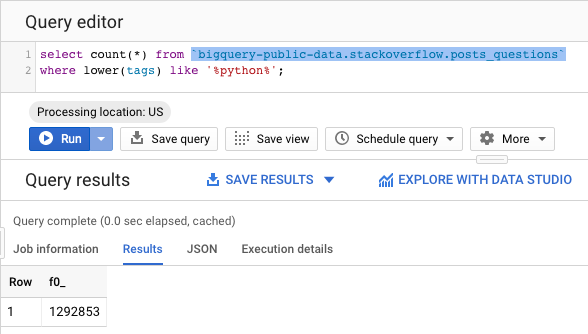
\includegraphics[width=12cm]{src/figuras/cap-introducao/number-python-questions-sof.png}
\caption{Total de perguntas sobre Python no \textit{StackOverFlow} até 11 de junho de 2019. Google and the Google logo are registered trademarks of Google LLC, used with permission.}
\label{fig:bigquery-total-questions-python-stackoverflow}
\end{figure}

\begin{figure}[h]
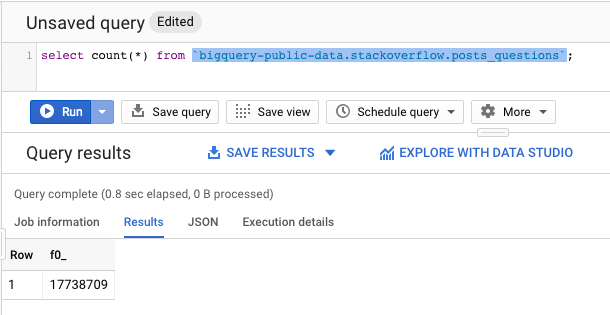
\includegraphics[width=12cm]{src/figuras/cap-introducao/number-questions-sof.png}
\caption{Total de perguntas no \textit{StackOverFlow} até 11 de junho de 2019. Google and the Google logo are registered trademarks of Google LLC, used with permission.}
\label{fig:bigquery-total-questions-stackoverflow}
\end{figure}

A partir de 2014, o \textit{Stackoverflow} tornou os dados abertos. Através do site \cite{sof-2019}, é possível obter os dados anônimos das perguntas e respostas feitas pelos usuários. Conforme \cite{Wang-quora:2013}, estes dados foram curados e organizados pela comunidade. Isto torna esta base relevante para áreas de pesquisa como inteligência artificial, mais especificamente a área de \gls{ml}. 

\cite{Allamanis-bimodal-source-code-natural-language:2015} utilizou os dados do \textit{Stackoverflow} para criar um \gls{modelo} capaz de recuperar um trecho de código-fonte dado uma descrição em linguagem natural. Neste trabalho, criou-se uma \gls{representacao-distribuida} dos trechos de código-fonte e da linguagem natural e as combinou utilizando modelos aditivos e multiplicativos para classificar os pares de trechos de código-fonte e questões do \textit{Stackoverflow}. Já \cite{iyer-etal-2016-summarizing} utilizou uma rede \acrfull{lstm} com \gls{mecanismo-atencao} no problema de recuperar trecho de código-fonte a partir de uma questão.

Tanto o trabalho de \cite{Allamanis-bimodal-source-code-natural-language:2015} e \cite{iyer-etal-2016-summarizing} coletaram questões 







%% ------------------------------------------------------------------------- %%
\section{Considerações Preliminares}
\label{sec:consideracoes_preliminares}

lalalalala


%% ------------------------------------------------------------------------- %%
\section{Objetivos}
\label{sec:objetivo}

lalalalala

%% ------------------------------------------------------------------------- %%
\section{Contribuições}
\label{sec:contribucoes}

lalala

%% ------------------------------------------------------------------------- %%
\section{Organização do Trabalho}
\label{sec:organizacao_trabalho}

No Capítulo~\ref{cap:trabalhos-relacionados}, apresentamos os conceitos e trabalhos relacionados ao problema de perguntas e respostas em processamento de linguagem natural. No capítulo~\ref{cap:problema}, discutimos o problema de pesquisa proposto para o presente trabalho, a arquitetura proposta e apontamos detalhes dos dados utilizados pertinentes a pesquisa. 
No capítulo~\ref{cap:resultados-preliminares}, exibimos os resultados preliminares da arquitetura proposta utilizando os dados do \cite{yao-2018}. E também discutimos as principais dificuldades encontradas para adaptar a arquitetura do \cite{feng-2015} para resolver problema de pares de perguntas e códigos-fontes. Já no capítulo~\ref{cap:cronograma}, temos as considerações finais, proposta do cronograma e os próximos passos da pesquisa.
